\chapter{Konzeption und theoretische Grundlagen}
\label{cha:theoGrundlagen}

\section{Android App-Entwicklung}
Android ist ein auf dem Linux Kernel basierendes mobiles Betriebssystem. Zur
Zeit wird Android von Google entwickelt und zielt auf Geräte ab, die über einen
Touchscreen bedient werden. Dazu zählen Smartphones, Tablets und neuerdings auch
Smartwatches. Wie üblich bei auf Linux basierenden Betriebssystemen, ist auch
der Android Quellcode unter der \Fachbegriff{open source} Lizenz frei verfügbar.
Der Funktionsumfang des Betriebssystems lässt sich durch Apps beliebig
erweitern. Diese Apps können vom Benutzer aus dem \Fachbegriff{Google Play
Store} bezogen werden. Der \Fachbegriff{Play Store} stellt die zentrale App
dar, in der alle Apps katalogisiert sind die mithilfe des \Fachbegriff{Android
SDK} entwickelt wurden. \\
Das \Fachbegriff{Android Software Development Kit} bietet neben verschiedenen
Entwicklungswerkzeugen auch eine eigene Entwicklungsumgebung an. Zu den
verschiedenen Entwicklungswerkzeugen zählen unter anderem ein Debugger, die
Android Bibliotheken und ein Emulator der verschiedene mobile Endgeräte zu
Testzwecken emulieren kann. Dieser Emulator ermöglicht das Testen von Android
Applikationen falls kein physisches Gerät zur Verfügung steht. Die Kommunikation
mit physischen Geräten, beispielsweise um das Debugging von Apps auf dem Gerät
zu ermöglichen, findet über die Android Debug Bridge (ADB) statt. \\
Android Applikationen werden in \Fachbegriff{Java} entwickelt. Java ist eine 
objektorientierte Programmiersprache.
Java Quellcode wird vom Java Compiler in Bytecode umgewandelt, welcher
nicht wie bei anderen Programmiersprachen üblich direkt durch Hardware ausgeführt
wird, sondern auf einer virtuellen Maschine (der Java Virtual Machine) läuft.
Dies sorgt für die oft beworbene Plattformunabhängigkeit von Java. Ob Windows,
Mac, Linux oder mobile Betriebssysteme wie z.B Android, das Java Prinzip „Write
once run anywhere“ bringt Java auf mehr als 50 Mio. PCs und Milliarden von verschiedensten
Geräten weltweit.\footcite{sierra2006} \\
Die Entwicklung mit dem Android SDK unterscheidet sich nur an manchen Stellen
von klassischer Java Entwicklung. Viele native Java Bibliotheken können auch in
der Android Entwicklung eingesetzt werden. Die Entwicklung von Oberflächen
unterschiedet sich jedoch etwas von der klassischen Oberflächenentwicklung mit
\Fachbegriff{Java Swing}. Android Oberflächen werden in sogenannte
\Fachbegriff{Activities} unterteilt. Üblicherweise ist jeder
\Fachbegriff{Activity} eine bestimmte Oberfläche zugeordnet. Mithilfe der
verschiedenen \Fachbegriff{Activities} wird in erster Linie die Navigation
innerhalb der App gesteuert. Die \Fachbegriff{Activities} reagieren auf Gesten
und Tastendrücke des Benutzers. Sollte also ein Benutzer beispielsweise den
\Fachbegriff{Zurück} Button auf seinem Gerät drücken, so wechselt die App auf
die zuvor angezeigte \Fachbegriff{Activity}. \Fachbegriff{Activities} können
sich auch gegenseitig aufrufen und stellen somit
den Navigationsfluss innerhalb der App sicher.\footcite{kuenneth2012android}

\section{Verschiedene Lösungsmöglichkeiten}
Die Anzeige des readmore.de Forums in einer Android App ist über mehrere Wege
möglich. In Vorüberlegungen zu dieser Arbeit wurden zwei sinnvolle Möglichkeiten
ausgewählt, die in den folgenden Unterkapiteln gegeneinander abgewogen werden.
Die erste Möglichkeit wäre die Manipulation der bestehenden Webseite mithilfe
von JavaScript und der Veränderung des CSS der Seite, die zweite Möglichkeit
wäre die Entwicklung einer eigenen serverseitigen API die die notwendigen
Informationen ausliest und über eine Server-Schnittstelle bereitstellt.
Möglichkeit zwei beeinhaltet die Entwicklung der App mit nativen Android
Komponenten.
\subsection{Manipulation der bestehenden Webseite}
Android bietet mit der \Fachbegriff{WebView} Komponente einen vollwertigen
Browser, der in einer Android App eingebettet werden kann. Dieser bietet auch
die Möglichkeit im Vollbildmodus zu laufen, sodass der Benutzer trotzdem das
Gefühl hat eine vollwertige App zu benutzen. Mithilfe von JavaScript ist es
möglich nur die für die mobile Nutzung notwendigen Komponenten einer Webseite
anzuzeigen. Durch die Veränderung des der Webseite zugrundeliegenden CSS, ist es
möglich das Design und die Anordnung der Komponenten für eine mobile Ansicht
anzupassen. \\
Vorteile der Lösung:
\begin{itemize}
  \item Die Oberfläche der App müsste nicht neu entwickelt werden. Die
  bestehenden Komponenten der Webseite müssen nur angepasst werden.
  \item Zeitersparnis durch die indirekte Verwendung der API von readmore.de.
  Login und erstellen von Posts findet direkt über die Webseite statt.
\end{itemize}
Nachteile der Lösung:
\begin{itemize}
  \item Komplizierte JavaScript Operationen um gewünschte Elemente auszuwählen.
  \item Obwohl nur die wichtigen Komponenten angezeigt werden, muss im
  Hintergrund die gesamte Webseite geladen werden. Dies führt zum einen zu einem
  erhöhten Datenverbrauch für Nutzer im Mobilfunknetzt, zum Anderen entstehen
  bei langsamen mobilen Datenverbindungen sehr hohe Ladezeiten für den Benutzer
  der App.
  \item Trotz der Anpassung auf eine mobile Webseite, fühlt sich die Benutzung
  einer WebView nicht wie eine native App an. Die Usability ist mit dieser
  Lösung zwar besser als zuvor, jedoch nicht auf dem Niveau einer nativen
  Android App.
  \item Komplexe JavaScript Operationen können auch mit einer schnellen
  Datenverbindung spürbare Verzögerungen für den Benutzer mit sich bringen.
\end{itemize}
\subsection{Entwicklung einer eigenen serverseitigen API}
Um die Daten im Forum von readmore.de wie z.B Foren, Threads und Beiträge
auszulesen soll eine eigene API entwickelt werden. Diese soll auf Anfrage die
gewünschten Informationen in einem weiterverarbeitbarem Format, wie z.B. JSON,
zur Verfügung stellen. Da die Analyse des HTML-Quellcodes der angeforderten
Seite auf dem Mobiltelefon unnötigen Datenverbrauch generieren würde, soll diese
API auf einem von überall aus erreichbaren Server laufen. Somit ist auch die
Wiederverwendbarkeit der API für andere Plattformen gewährleistet. Die App
soll im Anschluss mit nativen Android Komponenten entwickelt werden. \\
Vorteile der Lösung:
\begin{itemize}
  \item Entwicklung der App mit nativen Android Komponenten. Dadurch sehr gute
  Usability für den Benutzer.
  \item Da nur die wesentlichen Informationen an das Mobiltelefon übertragen
  werden, bleiben der Datenverbrauch sowie die Ladezeiten sehr niedrig.
  \item Entwickelte API setzt auf das weit verbreitete Format JSON. Dadurch ist
  die API plattformunabhängig einsetzbar und kann ohne Probleme weiterverwendet
  werden.
  \item Ressourcenauslastung des Mobiltelefons bleibt durch den Einsatz von
  nativen und schlanken Android Komponenten niedriger als in Möglichkeit 1
\end{itemize}
Nachteile der Lösung:
\begin{itemize}
  \item Login und Erstellen von Beiträgen müssen auf dem Smartphone simuliert
  werden
  \item Ausfall der API bedeutet Ausfall der App
  \item Es fallen Kosten für das Hosting des Servers an auf dem die API läuft
\end{itemize}
\subsection{Auswahl der Lösungsmöglichkeit}
Trotz Kosten durch das Hosting des Servers, fiel die Entscheidung auf die
Entwicklung einer eigenen API. Der hohe Datenverbrauch und vor allem die hohen
Ladezeiten bei der Verwendung einer WebView waren ausschlaggebend für die
Entscheidung. Diese Ladezeiten hätten die Usability vor allem bei mobilen
Datenverbindungen stark gesenkt. Daher wurde auf eine leichtgewichtige App mit
nativen Android Komponenten gesetzt, die über eine selbst entwickelte API nur
die nötigsten Daten zur Anzeige des Forums bereitgestellt bekommt. Der
Datenverbrauch und die Ladezeiten werden dadurch auf ein Minimum beschränkt.
\section{Eingesetzte Technologien}
\subsection{Jsoup}
Um die Informationen im readmore.de Forum, also verschiedene Foren und Beiträge,
auszulesen, wird die Java Bibliothek \Fachbegriff{jsoup} auf der
Serverseite eingesetzt.
\Fachbegriff{jsoup} ist eine Bibliothek mit der es möglich ist, HTML Dateien zu
parsen und die enthaltenen Informationen zu
extrahieren.\footnote{Quelle: http://jsoup.org/cookbook/} \Fachbegriff{jsoup}
bietet hierzu die Möglichkeit die Baumstruktur des eingelesenen HTML Dokuments zu durchlaufen und beispielsweise nach bestimmten Attributen zu filtern. Dazu
bietet die Bibliothek mit der sogenannten \Fachbegriff{Selektor Syntax} eine
Manipulationssprache um bestimmte Elemente im \Fachbegriff{DOM} des HTML
Dokument zu selektieren. Ein \Fachbegriff{DOM} ist in diesem Kontext die 
Baumstruktur in der das HTML Dokument strukturiert ist. \\
\subsection{Restlet}
Damit der Server auch von außen über HTTP Requests erreichbar ist, wurde das
Framework \Fachbegriff{Restlet} eingesetzt um eine \Fachbegriff{RESTful}
Serverkomponente bereit zu stellen. Das Programmierparadigma Representational
State Transfer (kurz: REST) beschreibt eine Serverkomponente die lediglich
unveränderte Seiteninhalte zum Abruf bereitstellt\footnote{Quelle:
http://restlet.com/products/restlet-framework/features/}. Die Kommunikation mit dieser Serverkomponente erfolgt über verschiedene HTTP-Methoden. Um beispielsweise
Daten vom Server abzurufen wird die Methode \Fachbegriff{GET} verwendet. Der Zustand am Server
wird dadurch nicht verändert. Restlet bringt eine fertige Serverkomponente mit
die nur noch an einem Port registriert werden muss. Über einen
\Fachbegriff{Router} werden dann Adressen verteilt die auf einzelne
\Fachbegriff{Restlets} verweisen. Wird also die URL eines \Fachbegriff{Restlets}
aufgerufen, reagiert das \Fachbegriff{Restlet} mit seiner Methode
\Code{handle()} auf die Anfrage. Dort werden dann die eventuellen Parameter des
GET-Requests ausgelesen, die Anfrage wird verarbeitet und anschließend wird die
angeforderte Ressource zurückgegeben. Nachfolgend ein Beispiel einer einfachen
\Fachbegriff{Restlet}-Serverkomponente mit einem Restlet.
\begin{lstlisting}[caption=Die Serverkomponente, label=komponente]
public class ReadmoreServer extends Application {
	private static ThreadsRestlet threadsRestlet;
	private static ForumRestlet forumRestlet;
	private static BeitragRestlet beitragRestlet;
	static {
		threadsRestlet = new ThreadsRestlet();
		forumRestlet = new ForumRestlet();
		beitragRestlet = new BeitragRestlet();
	}
	public static void main(String[] args) throws Exception {
		Component component = new Component();
		component.getServers().add(Protocol.HTTP, 8182);
		ReadmoreServer server = new ReadmoreServer();
		component.getDefaultHost().attach("", server);
		component.start();
	}
	public Restlet createInboundRoot() {
	    Router router = new Router(getContext());
	    router.attach("/threads", threadsRestlet);
	    router.attach("/forum", forumRestlet);
	    router.attach("/beitrag", beitragRestlet);
	    return router;
	  }
}
\end{lstlisting}
Wie in \ref{komponente} zu sehen, hört die Serverkomponente auf einen bestimmten
Port. In der Methode \Code{createInboundRoot()} wird mithilfe des \Code{Router}
die Adressen auf die die einzelnen Restlets reagieren festgelegt. Nachfolgend
ein einfaches \Fachbegriff{Restlet}
\begin{lstlisting}[caption=Ein einfaches Restlet, label=restlet]
public class ForumRestlet extends Restlet {
	@Override
    public void handle(Request request, Response response) {
		List<Forum> forum = getForum();
        String message = null;
        Gson gson = new Gson();
        message = gson.toJson(forum);
        response.setEntity(message, MediaType.TEXT_PLAIN);
    }
	private List<Forum> getForum() {
		ForenParser tp = new ForenParser();
		return tp.getForen();
	}
}
\end{lstlisting}
Die Methode \Code{handle(Request request, Response response)} legt beim Aufruf
des Restlets die \Fachbegriff{Response}, also die Antwort des Servers fest die
beim Aufruf zurückgegeben wird.
\subsection{Gson}
Das von Google entwickelte Framework \Fachbegriff{Gson} bietet die Möglichkeit
Java-Objekte vollautomatisch in das \Fachbegriff{JSON}-Format zu übertragen und
umgekeht \Fachbegriff{JSON}-Objekte in existierende Java-Objekte zu
transferieren.\footnote{https://sites.google.com/site/gson/gson-user-guide} 
\Fachbegriff{Gson} wird auf der Serverkomponente zur Erstellung der Antwort auf
GET Anfragen verwendet. 
\section{Konzeption des Servers}
Die Serverkomponente der Readmore App dient in erster Linie dem Auslesen der
sichtbaren Informationen im Forum von readmore. Dazu gehören die verschiedenen
Foren die in verschiedene Kategorien unterteilt sind, die Threads, also die
Einträge in jedem gewählten Forum und die einzelnen Beiträge auf jeder Seite
eines gewünschten Threads. 
\begin{figure*}[!htbp]
\centering
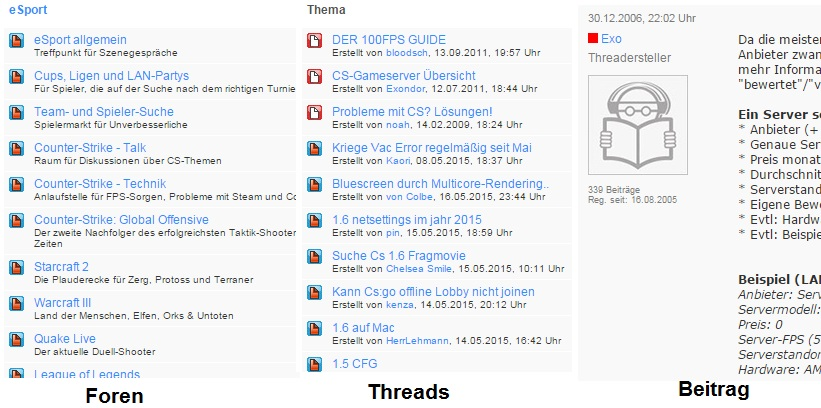
\includegraphics[width=\textwidth]{Bilder/ftb.jpg}
\caption[Foren, Threads und Beiträge auf Readmore]{Foren, Threads und Beiträge auf Readmore\protect\footnote{eigene Darstellung.} }
\label{dminfo}
\end{figure*}
Die App soll also nicht direkt mit readmore.de kommunizieren sondern bekommt
alle zur Anzeige des Forums relevanten Informationen in einem schnell zu
verarbeitenden Format. Dieses Vorgehen legt das aufwendige traversieren durch
den HTML-Code von readmore.de auf den Server um, und spart somit wertvolle
Ressourcen des Mobilgeräts ein. Der Server analysiert also das HTML der
gewünschten Forenseite auf readmore.de und extrahiert die relevanten
Informationen mithilfe von \Fachbegriff{Jsoup}. Ein vor allem im Android Bereich
sehr verbreitetes und gut verarbeitbares Format um strukturierte Daten darzustellen, 
stellt \Fachbegriff{JSON} dar. Daher erfolgt die Rückgabe der Daten vom Server 
im JSON Format. Bei der Rückgabe wird zwischen drei
verschiedenen Listen mit drei verschiedenen Datentypen unterschieden. \\
\begin{enumerate}
  \item Foren: Eine Liste mit allen Foren des readmore.de Forums
  \item Threads: Eine Liste mit allen Threads eines bestimmten Forums
  \item Beiträge: Eine Liste mit allen Beiträgen der gewählten Seite eines
  Threads
\end{enumerate}
Informationen die bei der Anfrage der Forenliste weitergegeben werden, sind:
\begin{itemize}
  \item Der Titel des Forums
  \item Die ID des Forums
  \item Die ID der Kategorie in der das Forum eingeteilt ist
  \item Die Beschreibung des Forums
\end{itemize}
Wird die Liste der Threads eines bestimmten Forums angefordert, werden folgende
Informationen weitergegeben:
\begin{itemize}
  \item Der Titel des Threads
  \item Die ID des Threads
  \item Die ID des Forums in dem der Thread sich befindet
  \item Die Anzahl der Seiten des Threads
\end{itemize}
Sollen alle Beiträge eines Threads zurückgegeben werden, enthält die Antwort des
Servers eine Liste mit \Code{Beitrag} Objekten. Diese Objekte enthalten folgende
Attribute:
\begin{itemize} 
  \item Der Inhalt des Beitrags
  \item Der Ersteller des Beitrags welcher sich aufteilt in:
  \begin{itemize}
    \item Die ID des Benutzers
    \item Der Anzeigename des Benutzers
    \item Der Link zum Avatar des Benutzers
  \end{itemize}
\end{itemize}
Wie in den Auflistungen zu sehen, werden hier nur die wesentlichen Informationen
über den Server übertragen. Da die übertragenen Daten nur im Textformat
übertragen werden, bleibt die übertragene Datenmenge minimal. Dadurch kann das
Laden von Foren, Threads und Beiträgen auf dem Mobiltelefon ohne zeitaufwändige
Ladezeiten geschehen. Der Zugriff auf den Server erfolgt über einen HTTP GET
Request. Hierbei werden die erforderlichen Parameter an die URL des Requests
angehängt. Wird beispielsweise eine Liste mit den Threads eines Forums
abgefragt, werden die Paramter \Code{forumId} und \Code{categoryId} an die URL
des GET Requests angehängt.
\section{Anforderungen an die Oberfläche}
Die große Herausforderung in dieser Studienarbeit liegt daran, die Informationen
des Forums in einem schnell verarbeitbaren Format darzustellen. Daher sollen
zunächst nur die wichtigsten Funktionen des Forums in der App abgebildet werden.
Zu den wichtigsten Funktionen zählen:
\begin{itemize}
  \item Die Anzeige aller Foren, Threads und Beiträge des gesamten Forums
  (lesen des Forums)
  \item Login aus der App heraus direkt via readmore.de
  \item Antworten in Threads aus der App heraus verfassen
  \item korrekte Darstellung des im Forum verwendeten BBCode, also der
  Formatierung für Zitate, Formatierung, Bilder und Links in den Beiträgen
\end{itemize}
\begin{figure*}[!htbp]
\centering
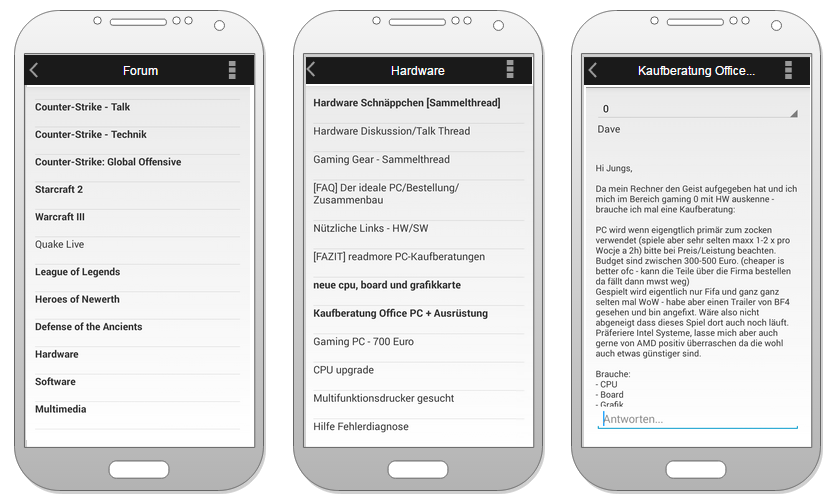
\includegraphics[width=\textwidth]{Bilder/mockups_oberflaeche.png}
\caption[Mockups der verschiedene Oberflächen der App]{Mockups der verschiedene Oberflächen der App
\protect\footnote{eigene Darstellung.} }
\label{dminfo}
\end{figure*}
Die höchste Priorität hat logischerweise das Lesen des Forums. Die Foren,
Threads und Beiträge sollen in drei unterschiedlichen Listen angezeigt werden.
Wird auf ein Eintrag in der Liste der Foren geklickt soll die entsprechende
Liste mit den Threads angezeigt werden. Ein Klick auf einen Thread soll die
Beiträge der ersten Seite des gewählten Threads darstellen. Außerdem sollen
innerhalb eines Threads die verfügbaren Seiten auswählbar sein. Die Darstellung
soll mit nativen Android Komponenten erfolgen.
Die Mockups enthalten in der Forenübersicht und der Threadübersicht jeweils
normal gedruckte Titel und fett gedruckte Titel. Falls der Benutzer in der App
eingeloggt ist, sollen fett gedruckte Titel ungelesene Threads oder Beiträge
symbolisieren. Normal gedruckte Titel symbolisieren, dass alle Beiträge und
Threads bereits gelesen wurden.
